% Settings for the default beamer theme
\documentclass[english, aspectratio=169]{beamer}
\usepackage[T1]{fontenc}
\usepackage[utf8]{inputenc}
\usepackage{tabularx}
\usepackage{babel}
\usepackage[ruled,vlined]{algorithm2e}
\SetAlgorithmName{Algoritmus}{algoritmus}{List of Algorithms}
\setcounter{secnumdepth}{3}
\setcounter{tocdepth}{3}

\makeatletter

\newcommand\makebeamertitle{\frame{\maketitle}}

% (ERT) argument for the TOC
\AtBeginDocument{%
  \let\origtableofcontents=\tableofcontents
  \def\tableofcontents{\@ifnextchar[{\origtableofcontents}{\gobbletableofcontents}}
  \def\gobbletableofcontents#1{\origtableofcontents}
}

% Theme settings
\usetheme{Frankfurt}
\usecolortheme{default}
\usefonttheme[onlymath]{serif}

% Template settings
\setbeamertemplate{navigation symbols}{}
\setbeamertemplate{blocks}[rounded][shadow=false]
\setbeamertemplate{title page}[default][colsep=-4bp, rounded=true, shadow=false]
\makeatother

\begin{document}

% Title page
\section{Bevezetés}
\title[]{Üzleti Intelligencia}
\subtitle{8. Előadás: Objektum detekció}
\author[Kuknyó Dániel]{Kuknyó Dániel\\Budapesti Gazdasági Egyetem}
\date{2023/24\\1.félév}
\makebeamertitle

% Table of contents slide
\begin{frame}
\tableofcontents{}
\end{frame}

% Table of contents of the current section
\begin{frame}
\tableofcontents[currentsection]
\end{frame}

\begin{frame}{Osztályozás}
\begin{columns}
\begin{column}{.5\textwidth}
Osztályozás esetén a neurális hálózat output rétegében minden lehetséges osztályhoz egy neuron tartozik. A neuronok azt a valószínűséget becsülik meg, hogy \textbf{az adott mintaegyed mekkora valószínűséggel esik a neuronhoz tartozó kategóriába}.\par\smallskip
Ez a \textbf{softmax} réteg, ahol az egyes neuronok aktivációs függvénye a softmax függvény. A softmax rétegben lévő neuronok outputjainak összege mindig $1$.
\end{column}
\begin{column}{.5\textwidth}
\begin{center}
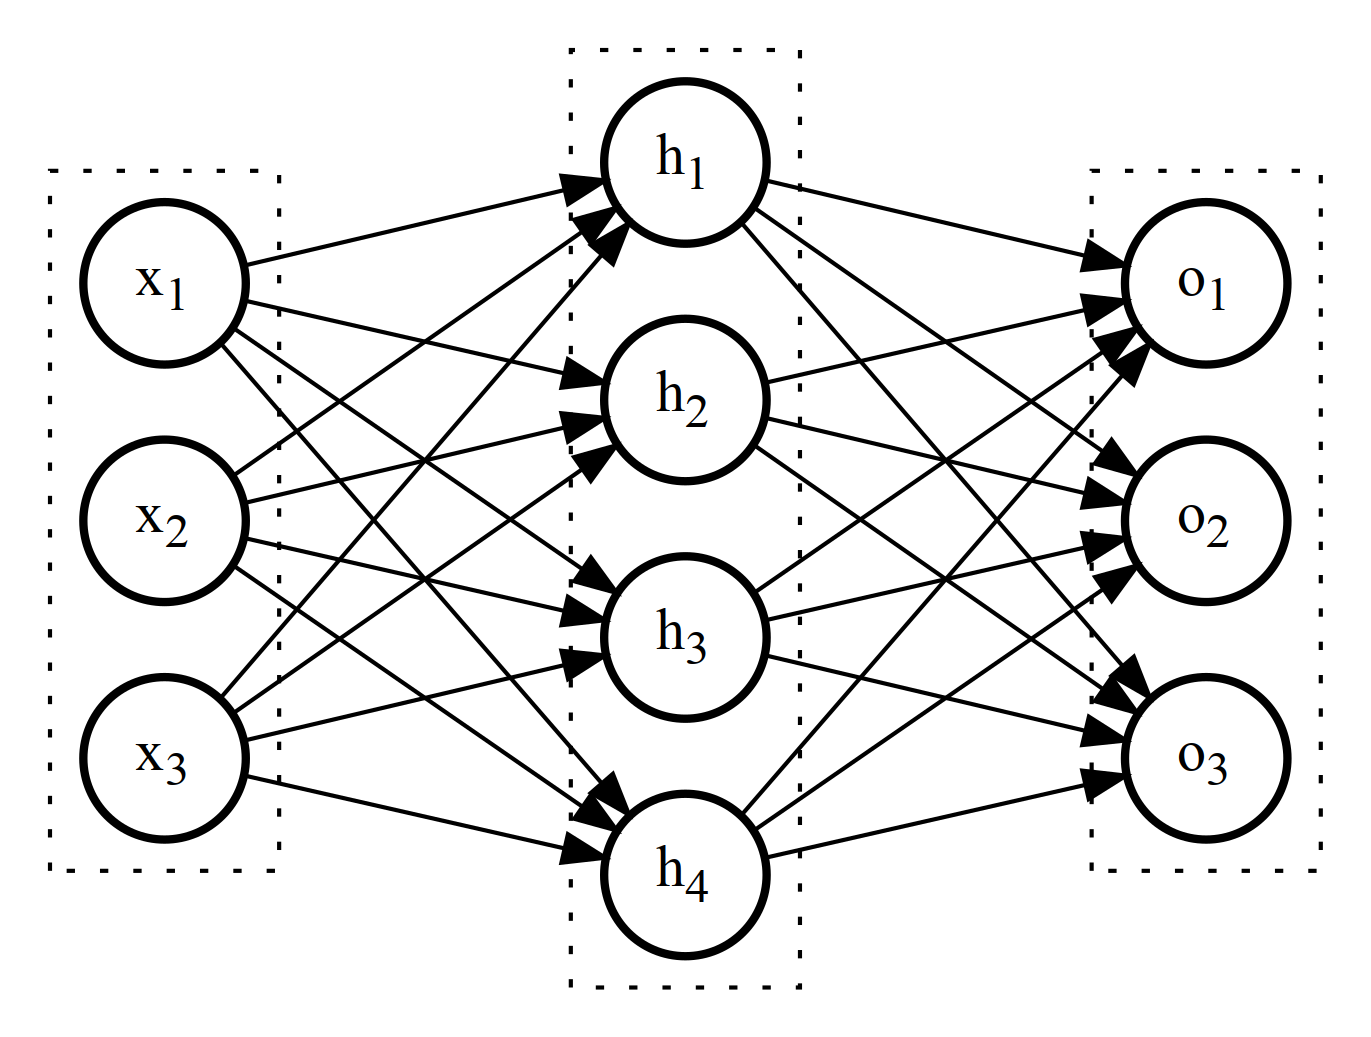
\includegraphics[width=7cm, keepaspectratio]{../../7_dl/doc/graphs/dl_1.png}
\end{center}
\end{column}
\end{columns}
\end{frame}

\begin{frame}{Predikció osztályozás esetén}
\begin{columns}
\begin{column}{.7\textwidth}
A legegyszerűbb módja az osztályozásnak, ha a hálózat outputként \textbf{összesen egy címkét} ad outputként, ami a predikciója az input képre (vagy adatra) vonatkozóan.\par\smallskip
Ebben az esetben a hálózat softmax rétege azt becsüli meg, hogy \textbf{mekkora válószínűséggel tartozik a mintaegyed a tanító osztályok valamelyikébe}. Például:
\[
\left[ macska: 0.9; kutya: 0.1 \right]
\]
Ezután az output úgy áll elő, hogy a hálózat \textbf{kiválasztja a legnagyobb valószínűségű osztályt} az $argmax$ operátorral, majd visszaadja a legnagyobb valószínűséghez tartozó címkét.
\end{column}
\begin{column}{.3\textwidth}
\begin{center}
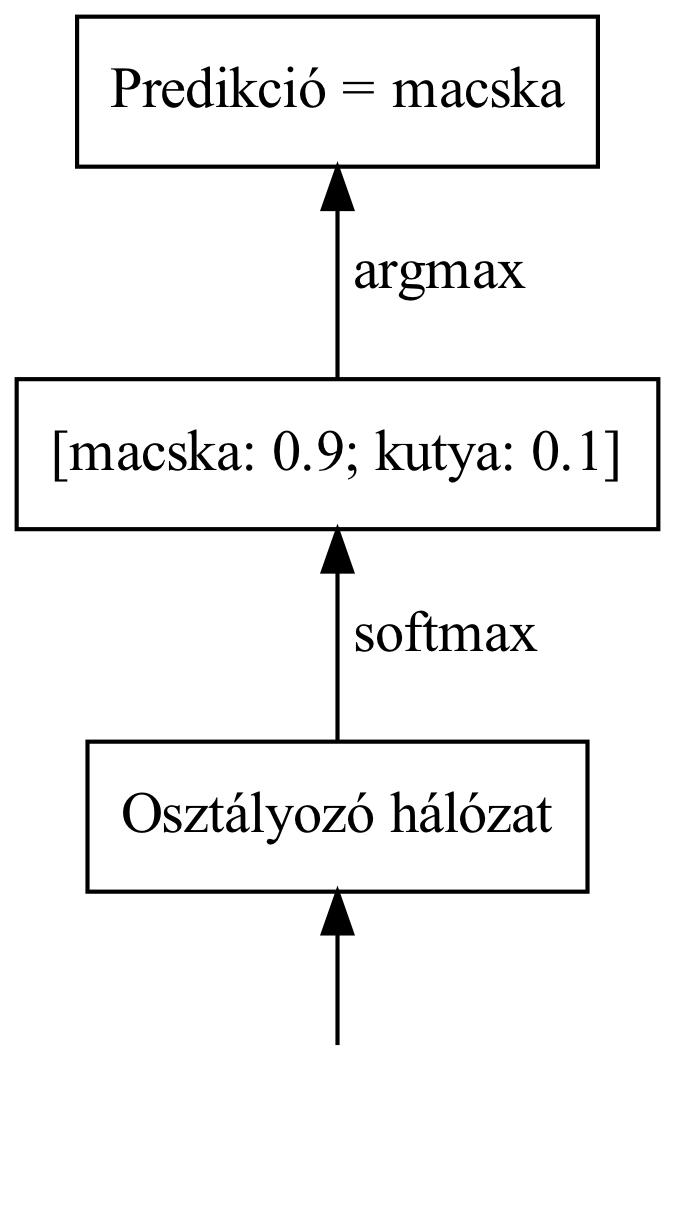
\includegraphics[height=5cm, keepaspectratio]{graphs/od_1.png}\\
\vspace{-0.7cm}
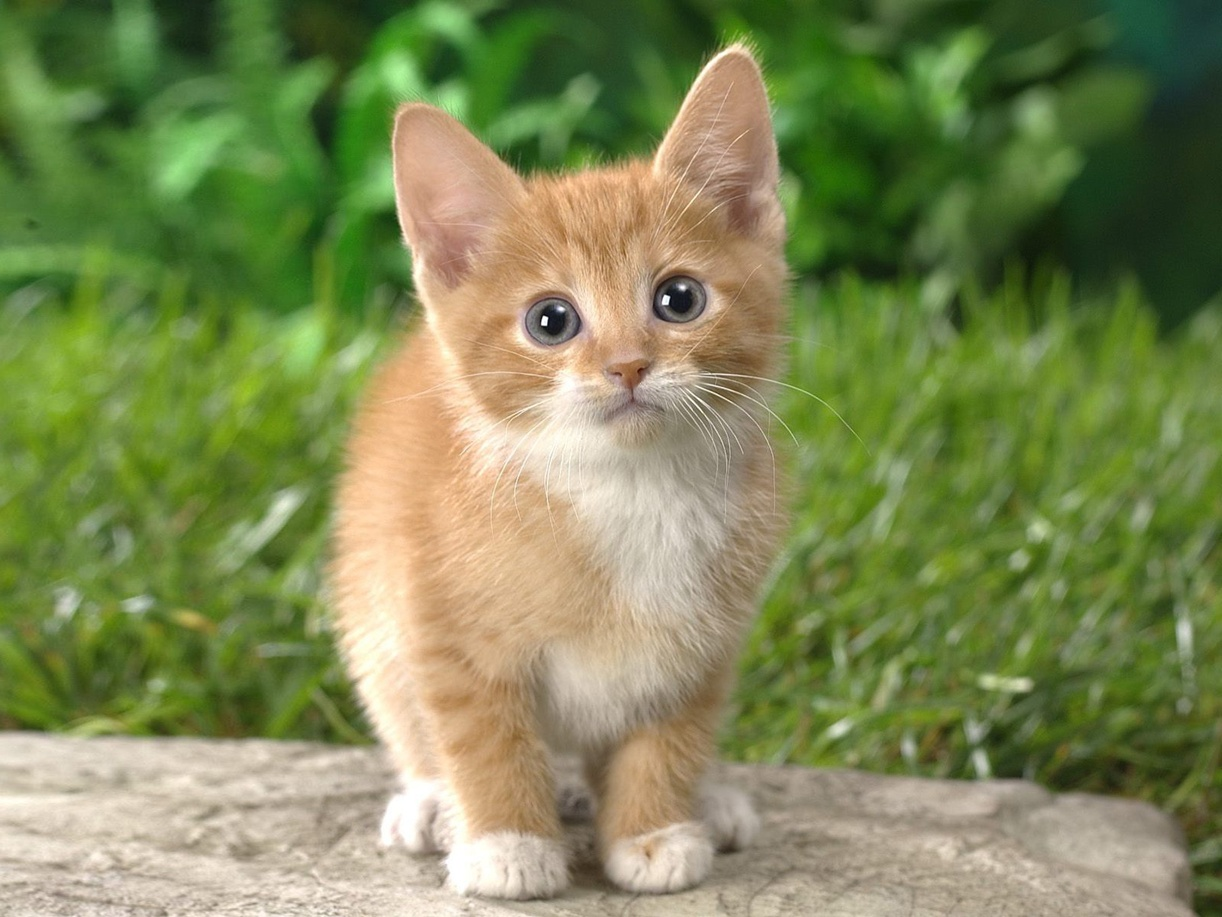
\includegraphics[height=2.5cm, width=2.5cm, keepaspectratio]{images/od_1.png}
\end{center}
\end{column}
\end{columns}
\end{frame}

\begin{frame}{Lokalizáció}
\begin{columns}
\begin{column}{.7\textwidth}
Az objektum lokalizáció feladata az osztályozás egy speciális esete. A lokalizáció problémájában nem csak azt kell megbecsülnie a neurális hálózatnak, hogy milyen objektum található egy képen, hanem meg is kell adnia az \textbf{objektum pozícióját azzal, hogy megadja a kereteződobozának koordinátáit}.\par\smallskip
Ebben az esetben a hálózat outputja nem csak egy címke, hanem a dobozt meghatározó négy koordináta is. Ezek a leggyakrabban:
\begin{itemize}
	\item $x$: A doboz bal felső sarkának $x$ koordinátája.
	\item $y$: A doboz bal felső sarkának $y$ koordinátája.
	\item $w$: A doboz szélessége (width).
	\item $h$: A doboz magassága (height).
\end{itemize}
\end{column}
\begin{column}{.3\textwidth}
\begin{center}
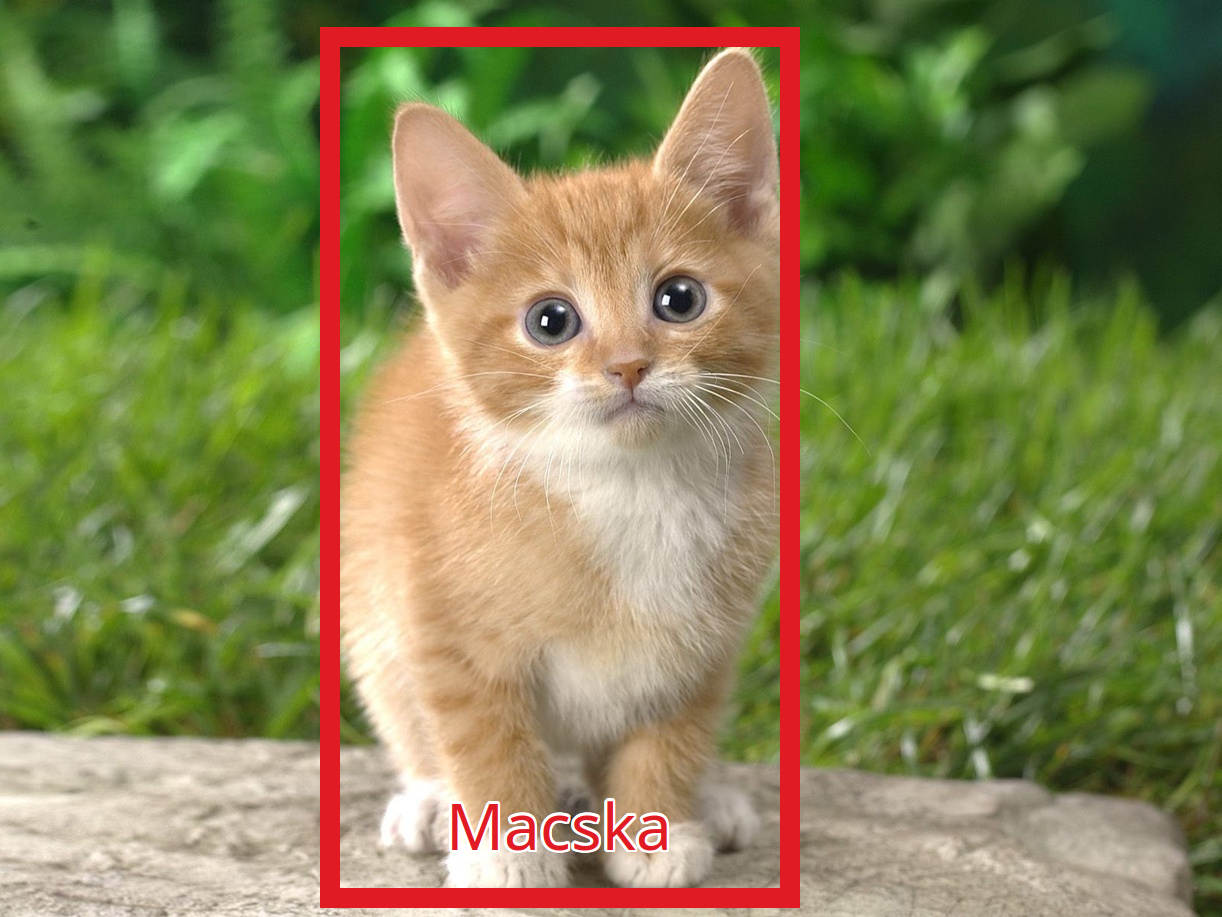
\includegraphics[width=4cm, keepaspectratio]{images/od_2.png}
\end{center}
\end{column}
\end{columns}
\end{frame}

\begin{frame}{Predikció lokalizáció esetén}
\begin{columns}
\begin{column}{.6\textwidth}
Lokalizáció esetén a neurális hálózat két részre ágazik, mivel két különböző feladatot kell elvégeznie:\par\smallskip
\textbf{Osztályozás}: ez megegyezik az osztályozó hálózat által végzett feladattal. A hálózat megbecsül egy valószínűségeloszlást, majd ebből kiválasztja a legnagyobb valószínűséghez tartozó osztályt, amit visszaad mint predikció.\par\smallskip
\textbf{Kereteződoboz predikciók}: a lokalizáció feladatához a neurális hálózatnak meg kell becsülnie az érdekelt régiók dobozainak koordinátáit. A neurális hálózat kiválasztja a becsült kereteződobozok közül azt, amelyik \textbf{a legnagyobb valószínűséggel tartalmazza a keresett objektumot}. 
\end{column}
\begin{column}{.4\textwidth}
\begin{center}
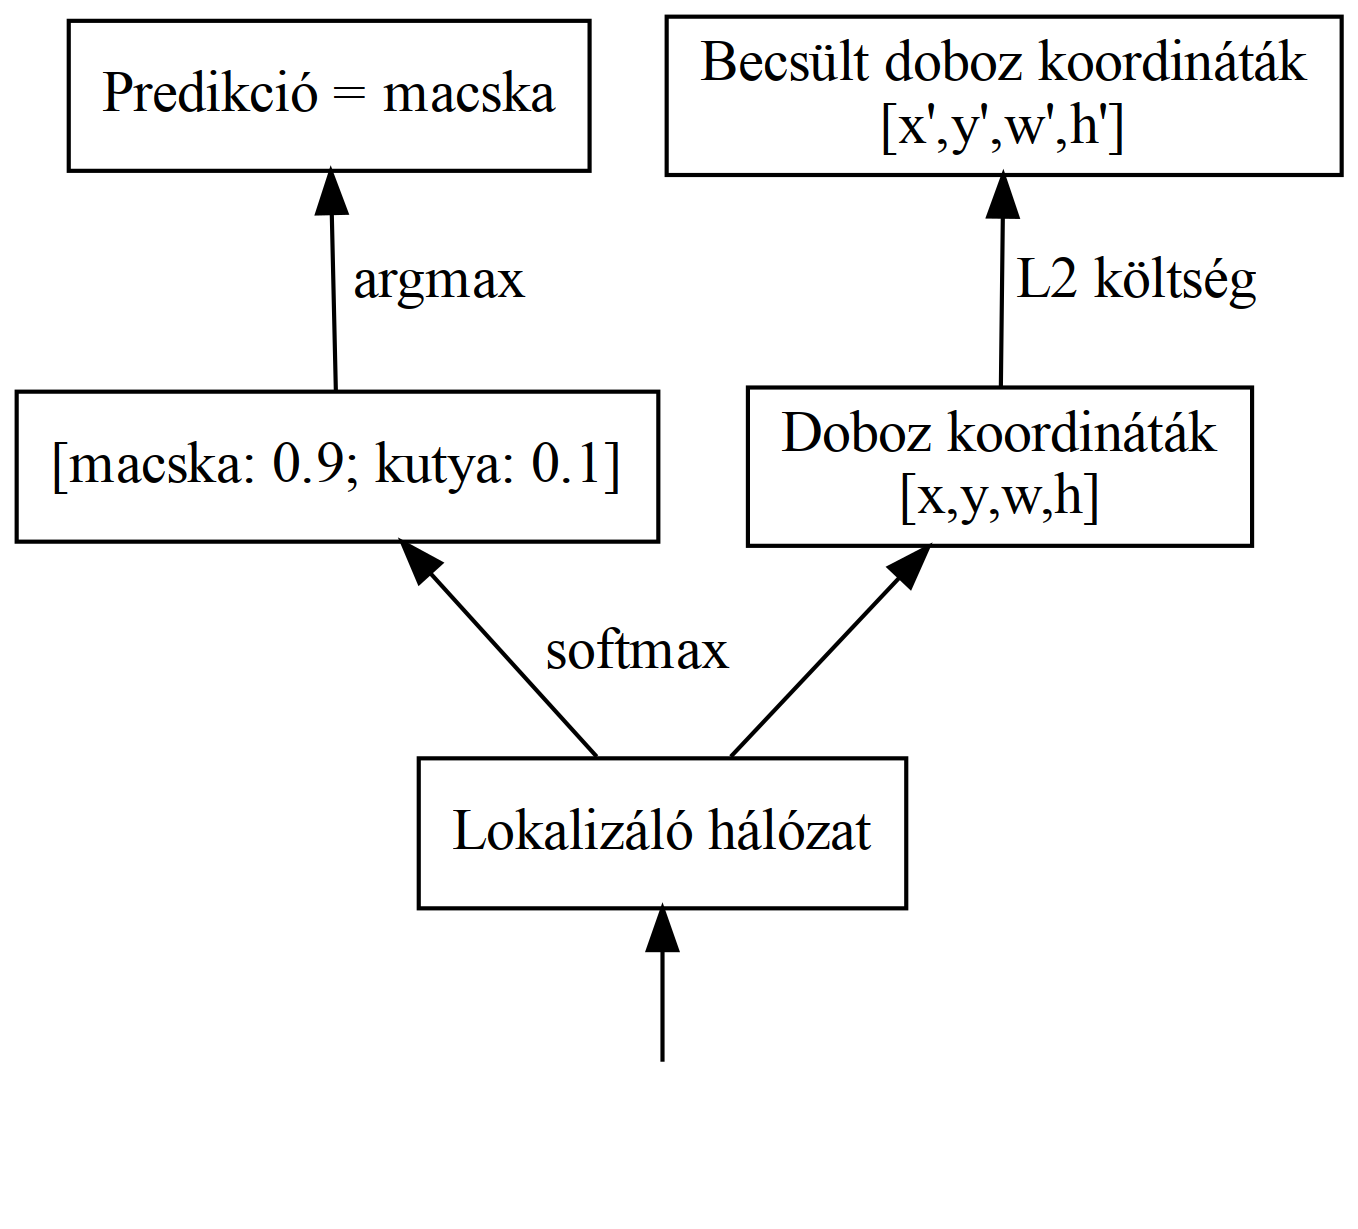
\includegraphics[height=5cm, keepaspectratio]{graphs/od_2.png}\\
\vspace{-0.7cm}
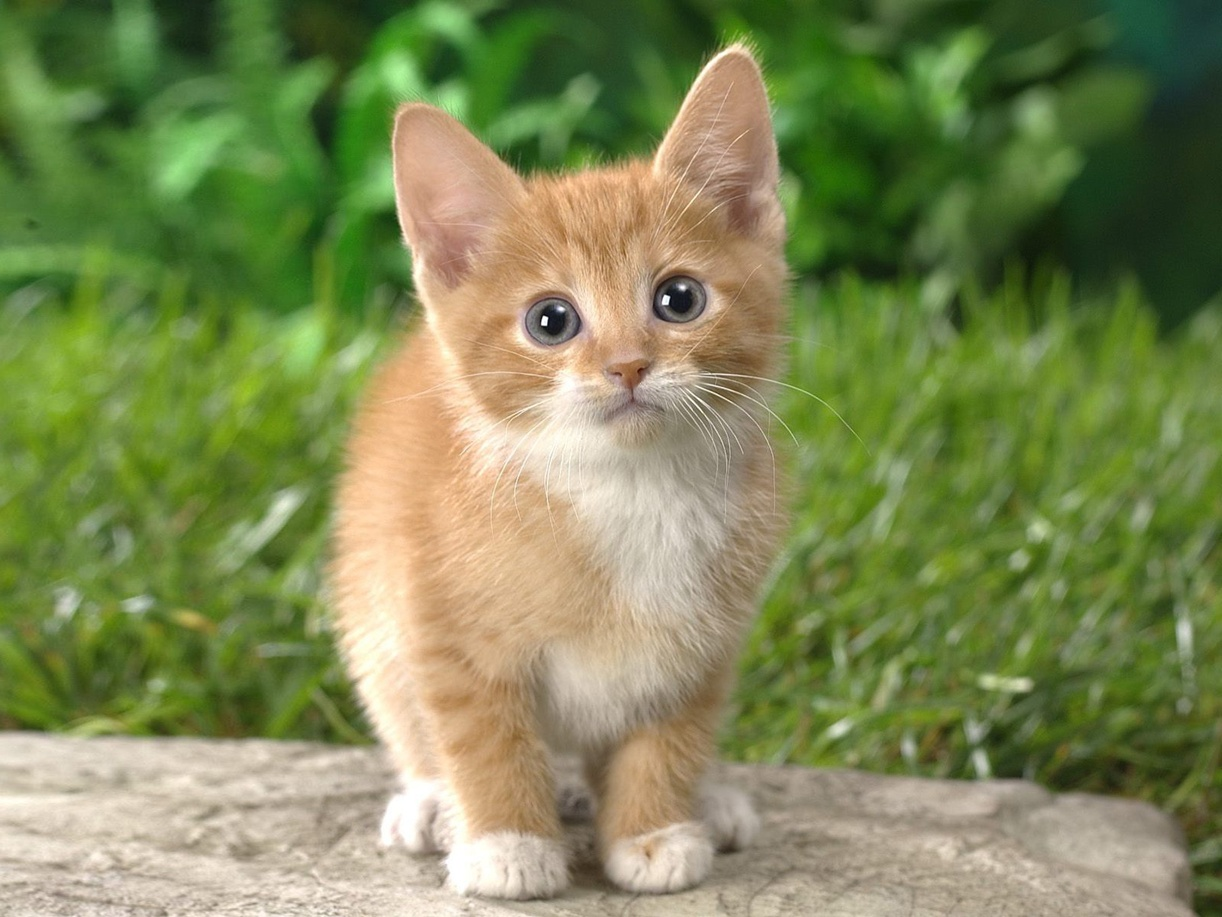
\includegraphics[height=2.5cm, width=2.5cm, keepaspectratio]{images/od_1.png}
\end{center}
\end{column}
\end{columns}
\end{frame}

\begin{frame}{Pontosság mérése kereteződobozokkal}
\begin{columns}
\begin{column}{.7\textwidth}
Mivel az objektum detekció egy felügyelt tanulási algoritmus, \textbf{szüksége van címkékre}. Ebben az esetben a címkék a valós osztályt és a kereteződoboz $x,y,w,h$ koordinátáit tartalmazzák.\par\smallskip
A jóságfüggvény $A$ valós és $B$ becsült kereteződoboz koordinátáit hasonlítja össze az IoU (metszet/unió) mérőszámmal:
\[
IoU=\frac{A \cap B}{A \cup B}
\]
Tehát minél jobban illeszkedik a becsült doboz a valósra, annál közelebb van a mérőszám $1$-hez. Ha a két doboznak nincs közös területe, $IoU=0$.
\end{column}
\begin{column}{.3\textwidth}
\begin{center}
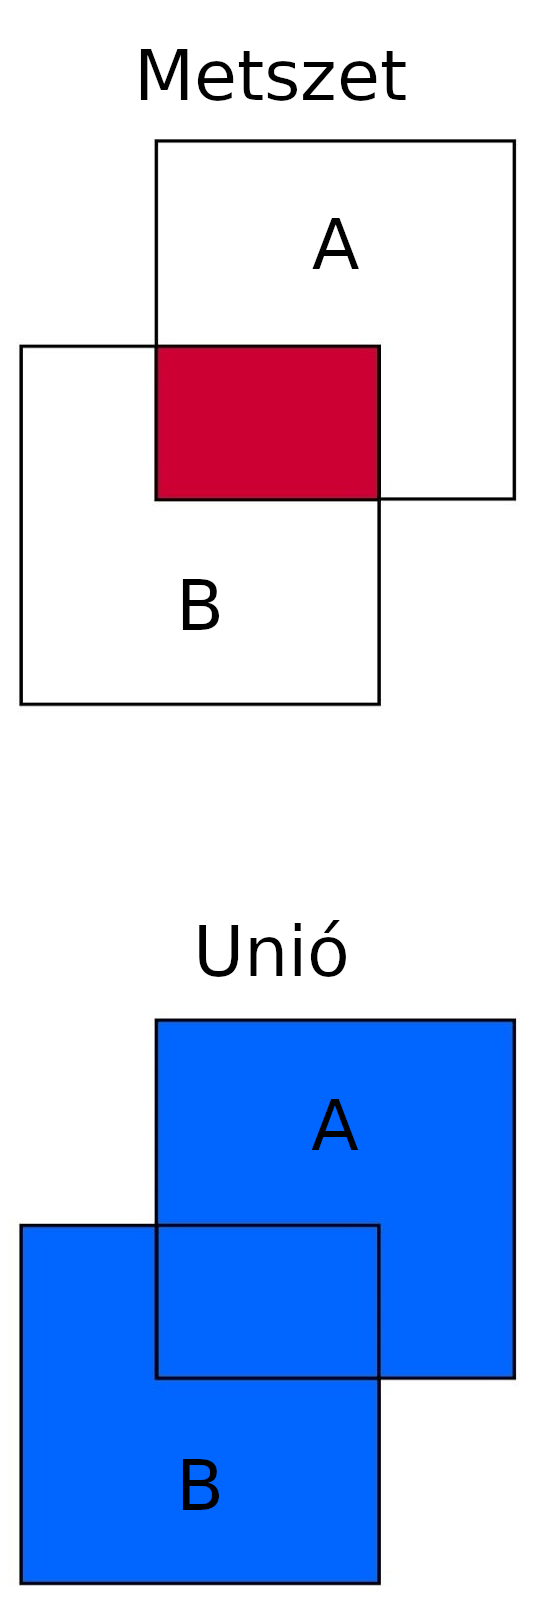
\includegraphics[height=7cm, width=7cm, keepaspectratio]{images/od_9.png}
\end{center}
\end{column}
\end{columns}
\end{frame}

\section{Objektum detekció}

\begin{frame}
\tableofcontents[currentsection]
\end{frame}

\begin{frame}{Objektum detekció}
\begin{columns}
\begin{column}{.5\textwidth}
Az objektum detekció a lokalizáció általánosítása több objektumra egyetlen képen belül. Ebben az esetben a neurális hálózat feladata \textbf{minden ismert objektum lokalizálása a képen}.\par\smallskip
Ebben az esetben a hálózat outputja minden egyes ismert objektumra: 
\begin{itemize}
	\item Az objektum becsült címkéje.
	\item Az objektum kereteződobozának $x,y,w,h$ koordinátái. 
\end{itemize}
Mivel az érdekelt objektumok száma képenként eltérő lehet, az \textbf{objektum detekciós hálózatok outputjainak számossága is képenként különbözik}!
\end{column}
\begin{column}{.5\textwidth}
\begin{center}
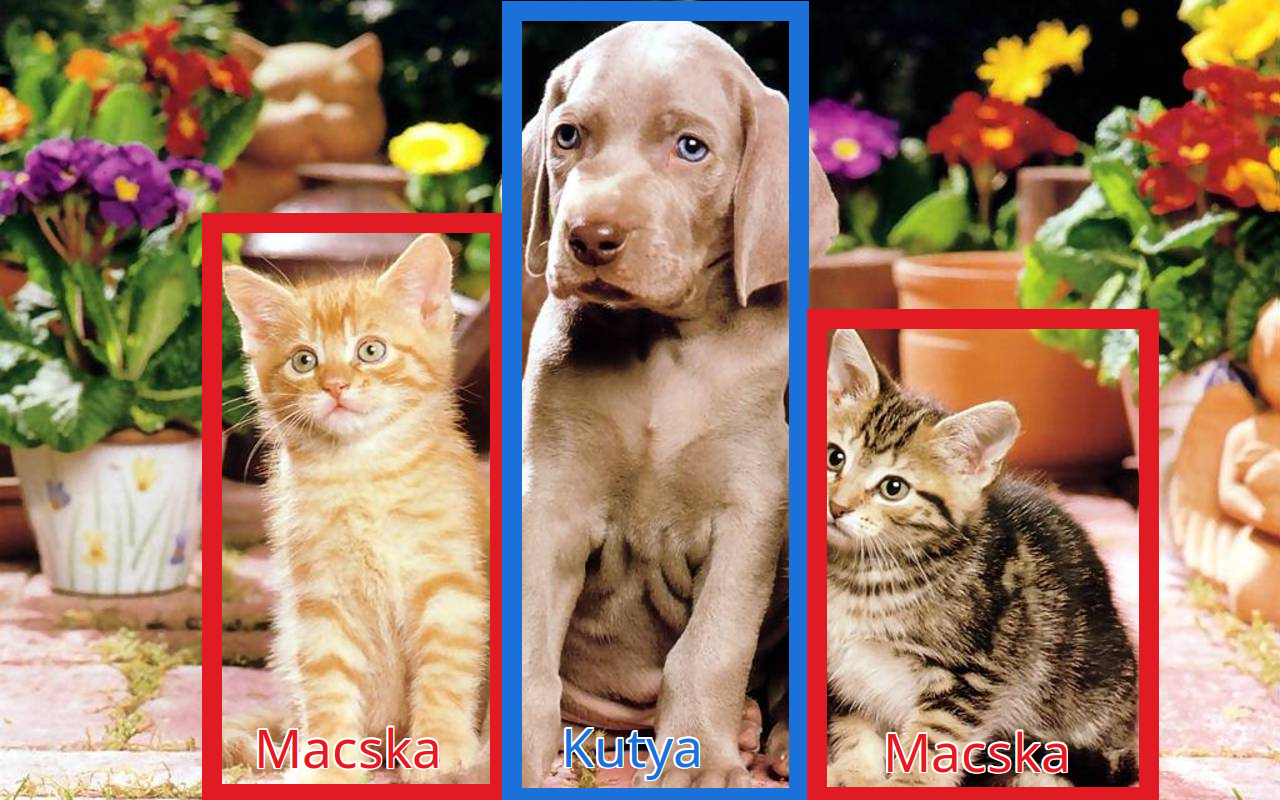
\includegraphics[width=7cm, keepaspectratio]{images/od_4.png}
\end{center}
\end{column}
\end{columns}
\end{frame}

\begin{frame}{Kezdeti detektor implementáció}
\begin{columns}
\begin{column}{.6\textwidth}
Az első objektum detektor modellek implementációi meglehetősen naívak voltak. Az eljárás szerint a modell \textbf{végigcsúsztat egy előre meghatározott méretű ablakot a képen}, és minden egyes általa meghatározott képről eldönti, \textbf{hogy háttér-e} ($bgr$) vagy valamelyik keresett osztályba tartozik-e:
\only<1>{
\[
output = [bgr: 0.8, kutya: 0.1, macska: 0.1]
\]
Ebben az esetben $\hat{y}=\underset{p}{argmax}(output)=bgr$, és az algoritmus eldobja a kereteződoboz predikcióját.
}
\only<2>{
\[
output = [bgr: 0.0, kutya: 0.01, macska: 0.99]
\]
Ebben az esetben $\hat{y}=\underset{p}{argmax}(output)=macska$, és a becsült kereteződoboz az, ahol a legnagyobb a keresett osztály valószínűsége.
}
\end{column}
\begin{column}{.5\textwidth}
\only<1>{
\begin{center}
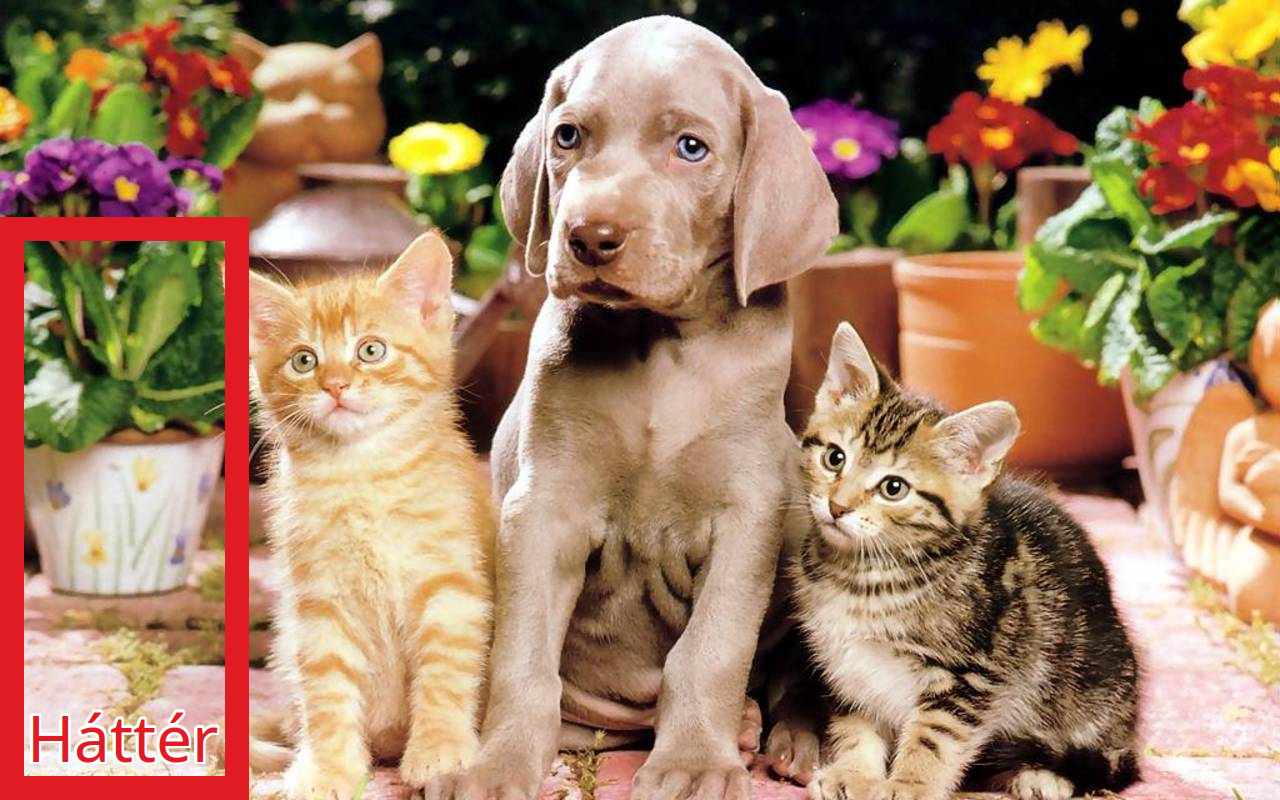
\includegraphics[width=7cm, keepaspectratio]{images/od_5.png}
\end{center}}
\only<2>{
\begin{center}
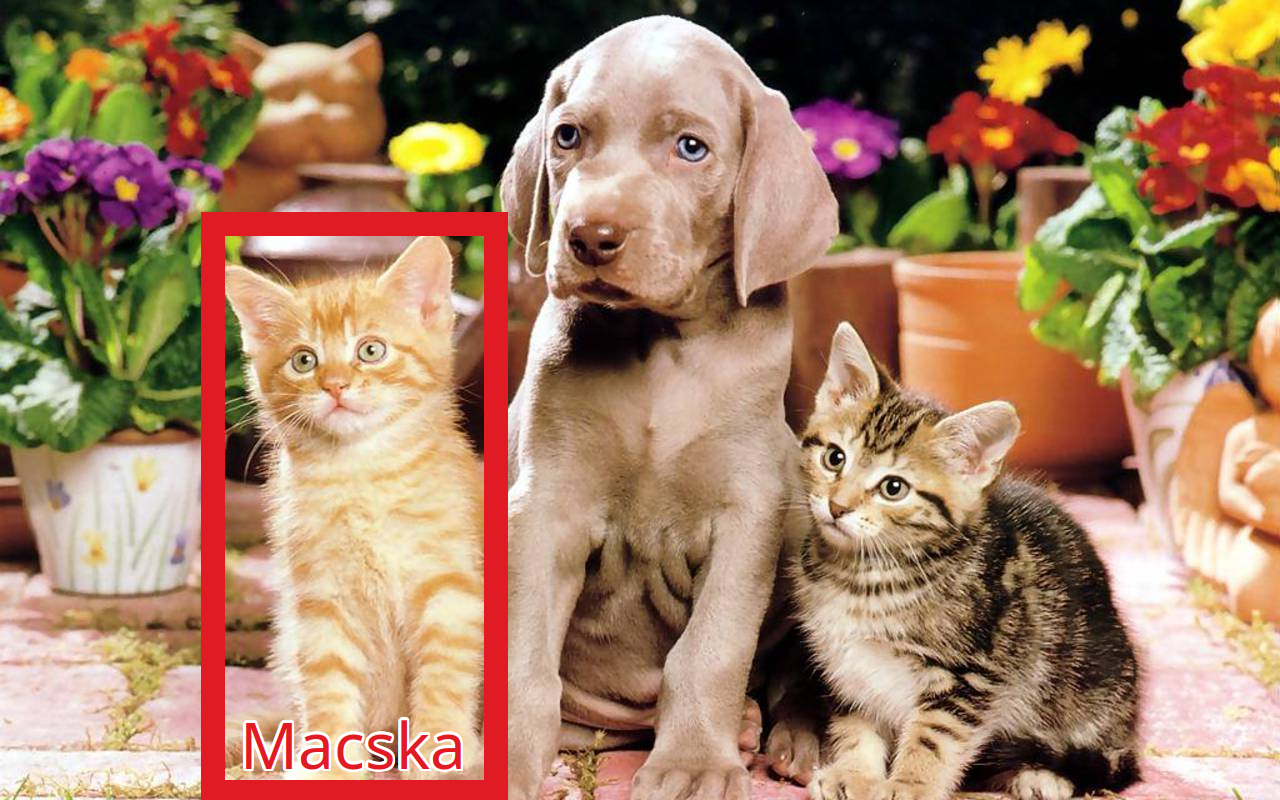
\includegraphics[width=7cm, keepaspectratio]{images/od_6.png}
\end{center}
}
\end{column}
\end{columns}
\end{frame}

\begin{frame}{Miért nem lehetséges ez az implementáció?}
\begin{columns}
\begin{column}{.7\textwidth}
Hány lehetséges kereteződoboz van egy $H \cdot W$ méretű képen?\par\medskip
Ha van egy $h \cdot w$ méretű kereteződoboz a lehetséges $x$ koordináták száma $W-w+1$, és a lehetséges $y$ koordináták száma $H-h+1$. A lehetséges megoldások száma egyetlen kereteződoboz méretre: $(W-w+1) \cdot (H-h+1)$.\par\medskip
Az összes lehetséges kereteződoboz méretre pedig:
\[
\sum_{h=1}^H \sum_{w=1}^W (W-w+1) \cdot (H-h+1) = \frac{H(H+1)}{2} \frac{W(W+1)}{2}
\]
Ez azt jelenti, hogy egy $800 \cdot 600$ méretű képre $\sim 58$ millió lehetséges kereteződoboz létezik.
\end{column}
\begin{column}{.3\textwidth}
\begin{center}
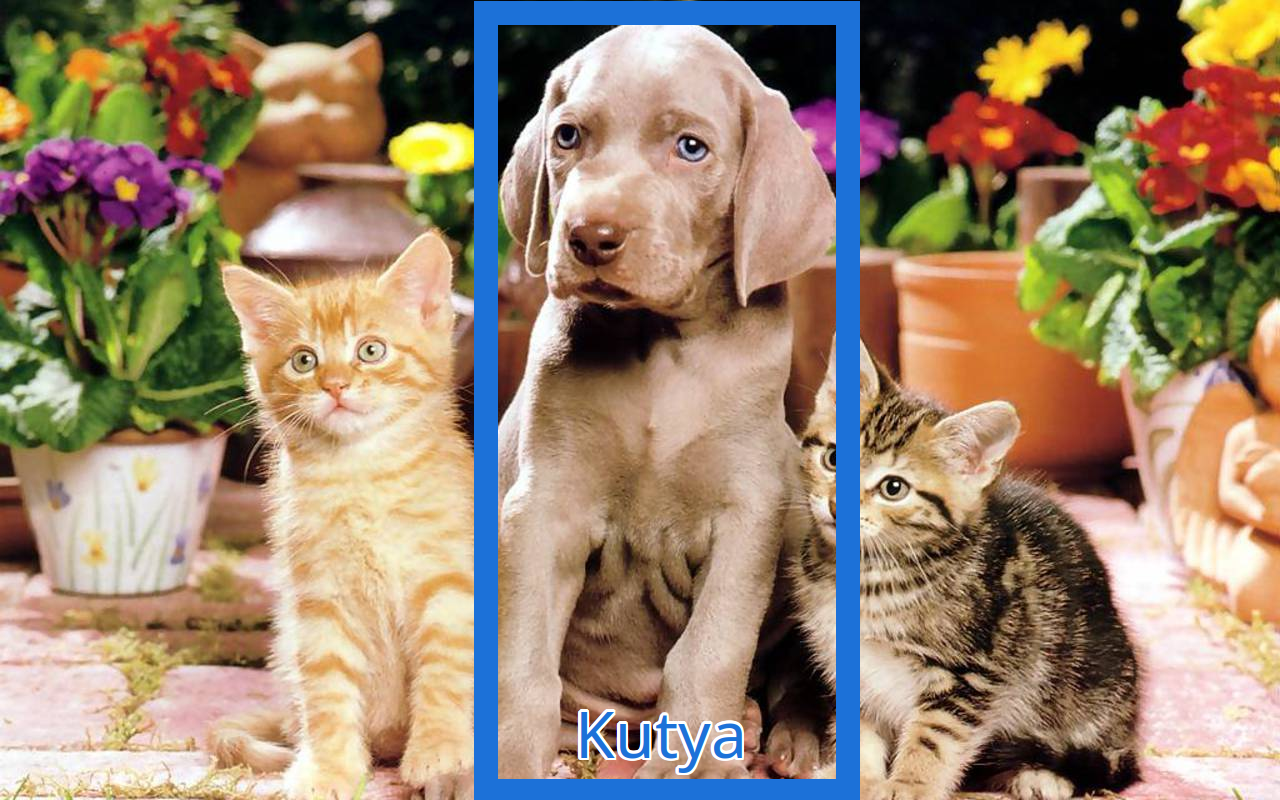
\includegraphics[height=7cm, width=4cm, keepaspectratio]{images/od_7.png}
\end{center}
\end{column}
\end{columns}
\end{frame}

\begin{frame}{Területi javaslatok}
\begin{columns}
\begin{column}{.6\textwidth}
Az eljárás ami meggyorsította a folyamatot a \textbf{területi javaslatok} algoritmusa volt.\par\smallskip
Ahelyett, hogy egy előre meghatározott méretű ablakot csúsztatna végig egy képen, a területi javaslatok algoritmusa megpróbálja a kép \textbf{pixeleit klaszterezni hasonlóság szerint}, ezzel területeket formázva.\par\smallskip
Később ezen \textbf{területeknek a kereteződobozai lesznek átadva egy osztályozó neurális hálózatnak} ami eldönti, hogy a keresett objektumok valamelyike mekkora valószínűséggel található meg a területen.
\end{column}
\begin{column}{.4\textwidth}
\begin{center}
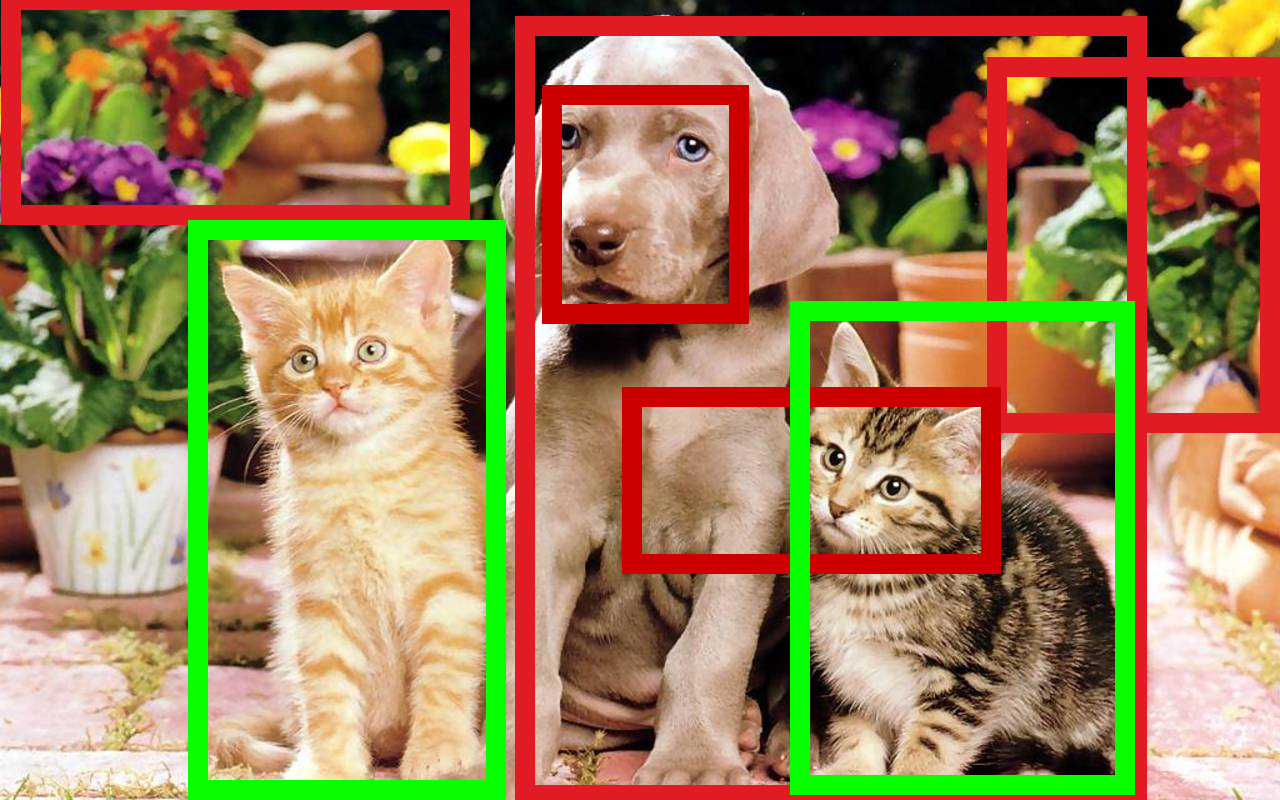
\includegraphics[height=7cm, width=6cm, keepaspectratio]{images/od_8.png}
\end{center}
\end{column}
\end{columns}
\end{frame}

\begin{frame}{Területi javaslatok szelektív kereséssel}
\begin{columns}[T]
\begin{column}{.8\textwidth}
\only<1->{A szelektív keresés egy potenciális objektum területeket javasoló algoritmus, ami jóval hatékonyabban képes működni, mint a csúszóablakos algoritmus:
\begin{enumerate}
	\item \textbf{Kép szegmentálása}: Az input kép pixeleinek csoportosítása szín, textúra és egyéb vizuális tulajdonságok szerint.
	\item \textbf{Régiók hasonlósága}: A különböző régiók összeolvasztása valamilyen hasonlósági mérték szerint.
	\item \textbf{Hierarchikus csoportosítás}: Az összeolvasztott régiók hierarchikus klaszterezése. 
	\item \textbf{Objektum javaslatok}: Objektum javaslatok halmazának elkészítése, amik területi javaslatként szolgálnak.
	\item \textbf{Objektum detekció}: A területi javaslatok átadódnak a neurális hálózatnak osztályozásra.
\end{enumerate}}
\end{column}
\begin{column}{.2\textwidth}
\vspace{-0.5cm}
\begin{center}
\only<1>{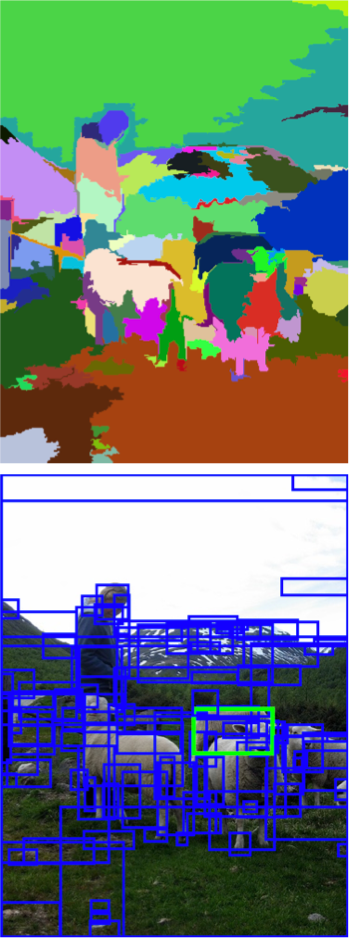
\includegraphics[height=7cm, keepaspectratio]{images/selective_search_1.png}}
\only<2>{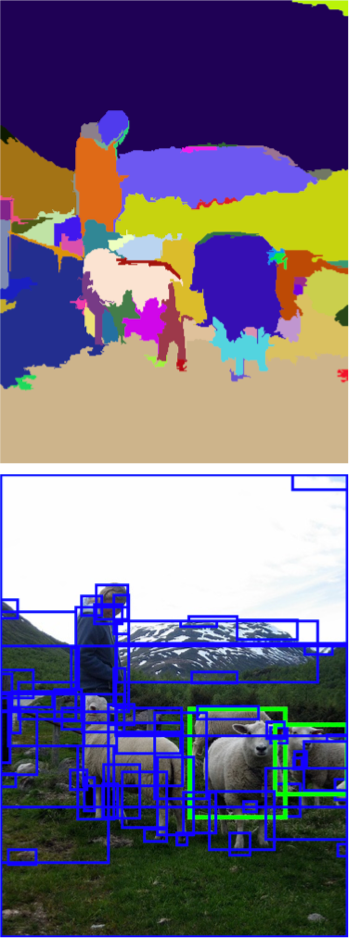
\includegraphics[height=7cm, keepaspectratio]{images/selective_search_2.png}}
\only<3>{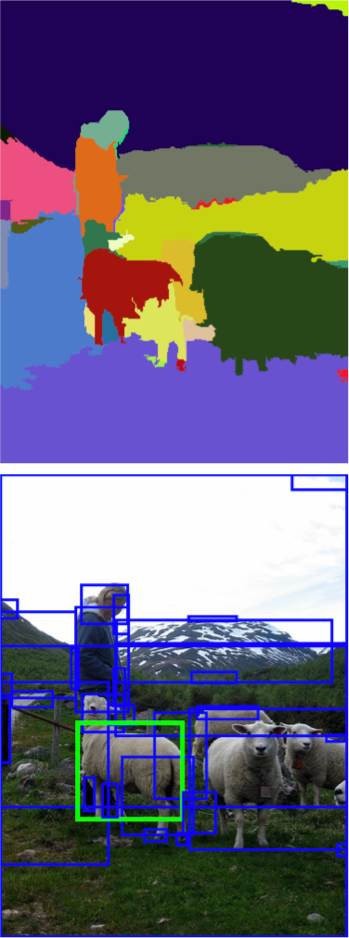
\includegraphics[height=7cm, keepaspectratio]{images/selective_search_3.png}}
\only<4>{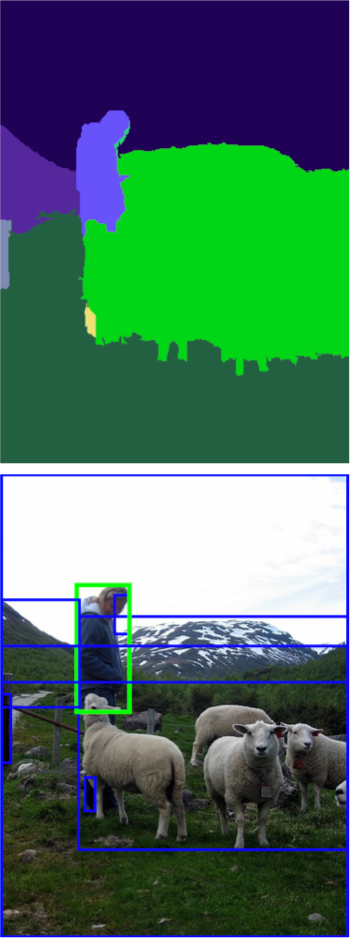
\includegraphics[height=7cm, keepaspectratio]{images/selective_search_4.png}}
\end{center}
\end{column}
\end{columns}
\end{frame}

\begin{frame}{Predikció objektum detekció esetén}
\begin{columns}
\begin{column}{.4\textwidth}
Az objektum detekció folyamata területjavasolással:
\begin{enumerate}
	\item A területjavasoló \textbf{kiválaszt érdekelt régiókat} a képről. Ezek lehetnek bármekkora méretűek.
	\item A javasolt régiók \textbf{fix méretűre vetítése}. Ez leggyakrabban $224 \cdot 224$ a gyors osztályozás miatt. 
	\item A lokalizációs hálózat \textbf{megbecsüli az osztályokat és a kereteződobozok koordinátáit} a vetített terület alapján
\end{enumerate}
\end{column}
\begin{column}{.6\textwidth}
\begin{center}
\only<1>{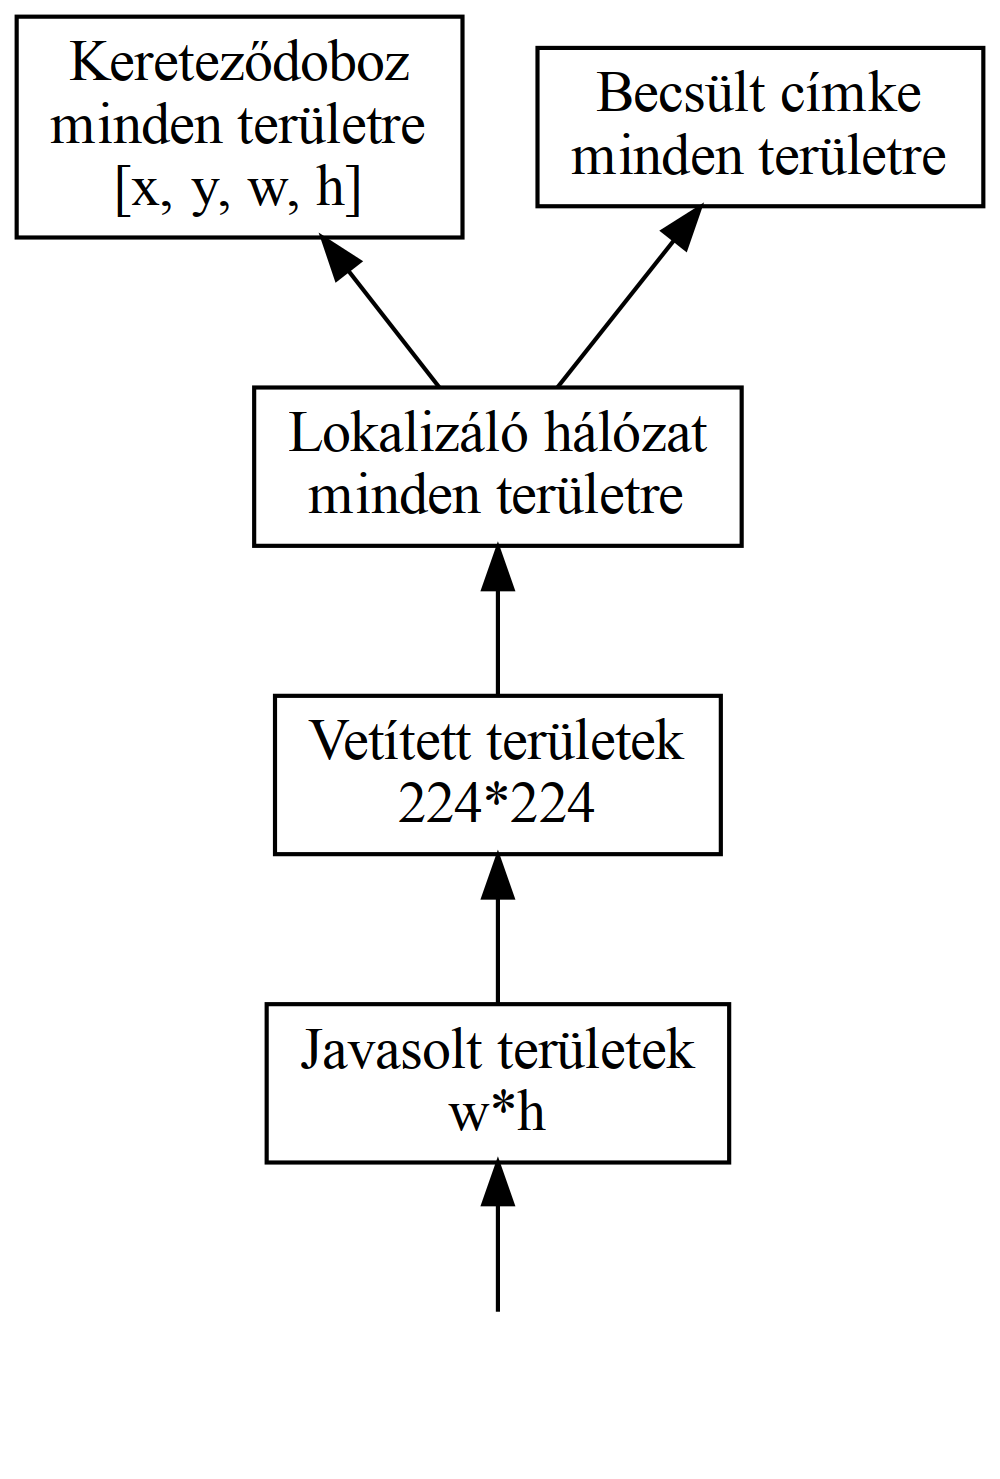
\includegraphics[height=6cm, width=7cm, keepaspectratio]{graphs/od_3.png}\\
\vspace{-0.7cm}
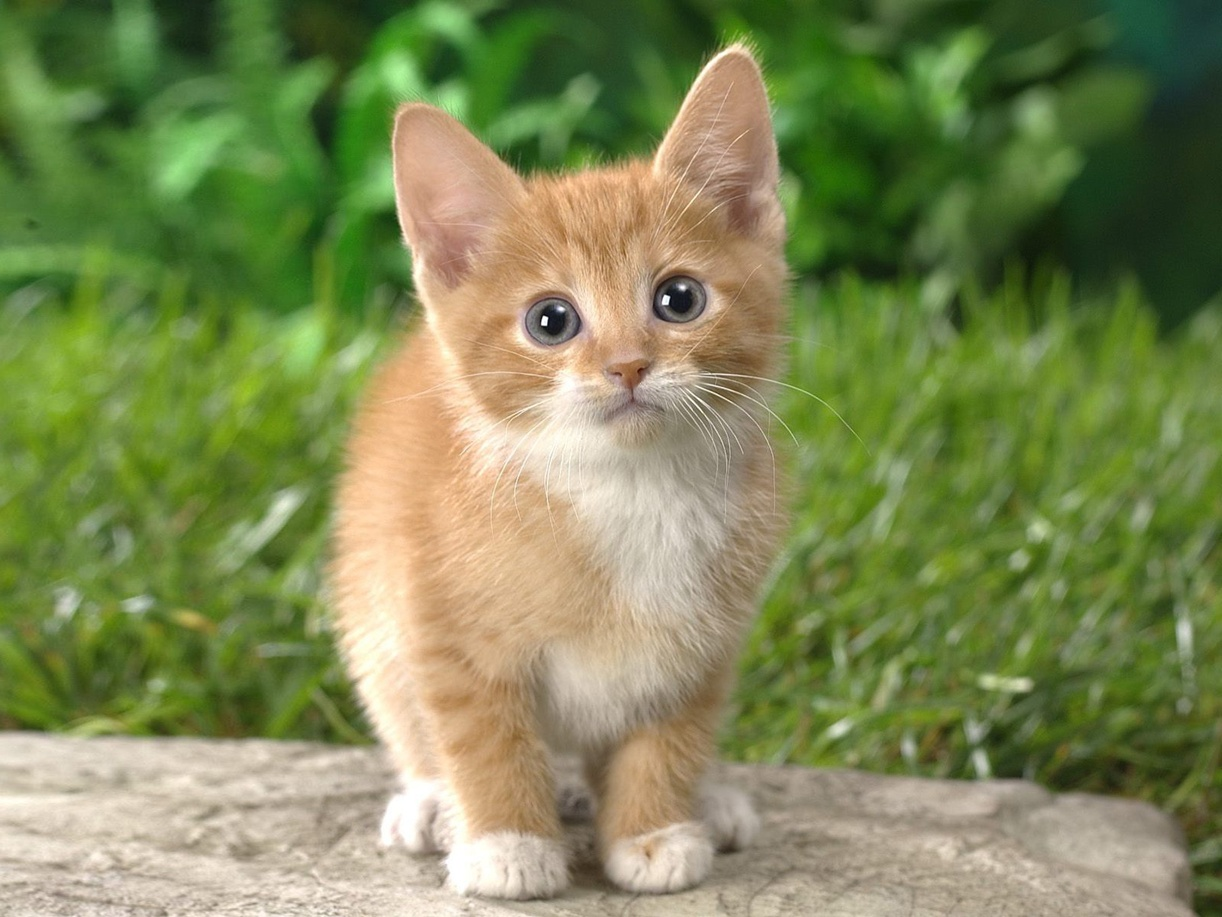
\includegraphics[height=1.5cm, keepaspectratio]{images/od_1.png}}
\only<2>{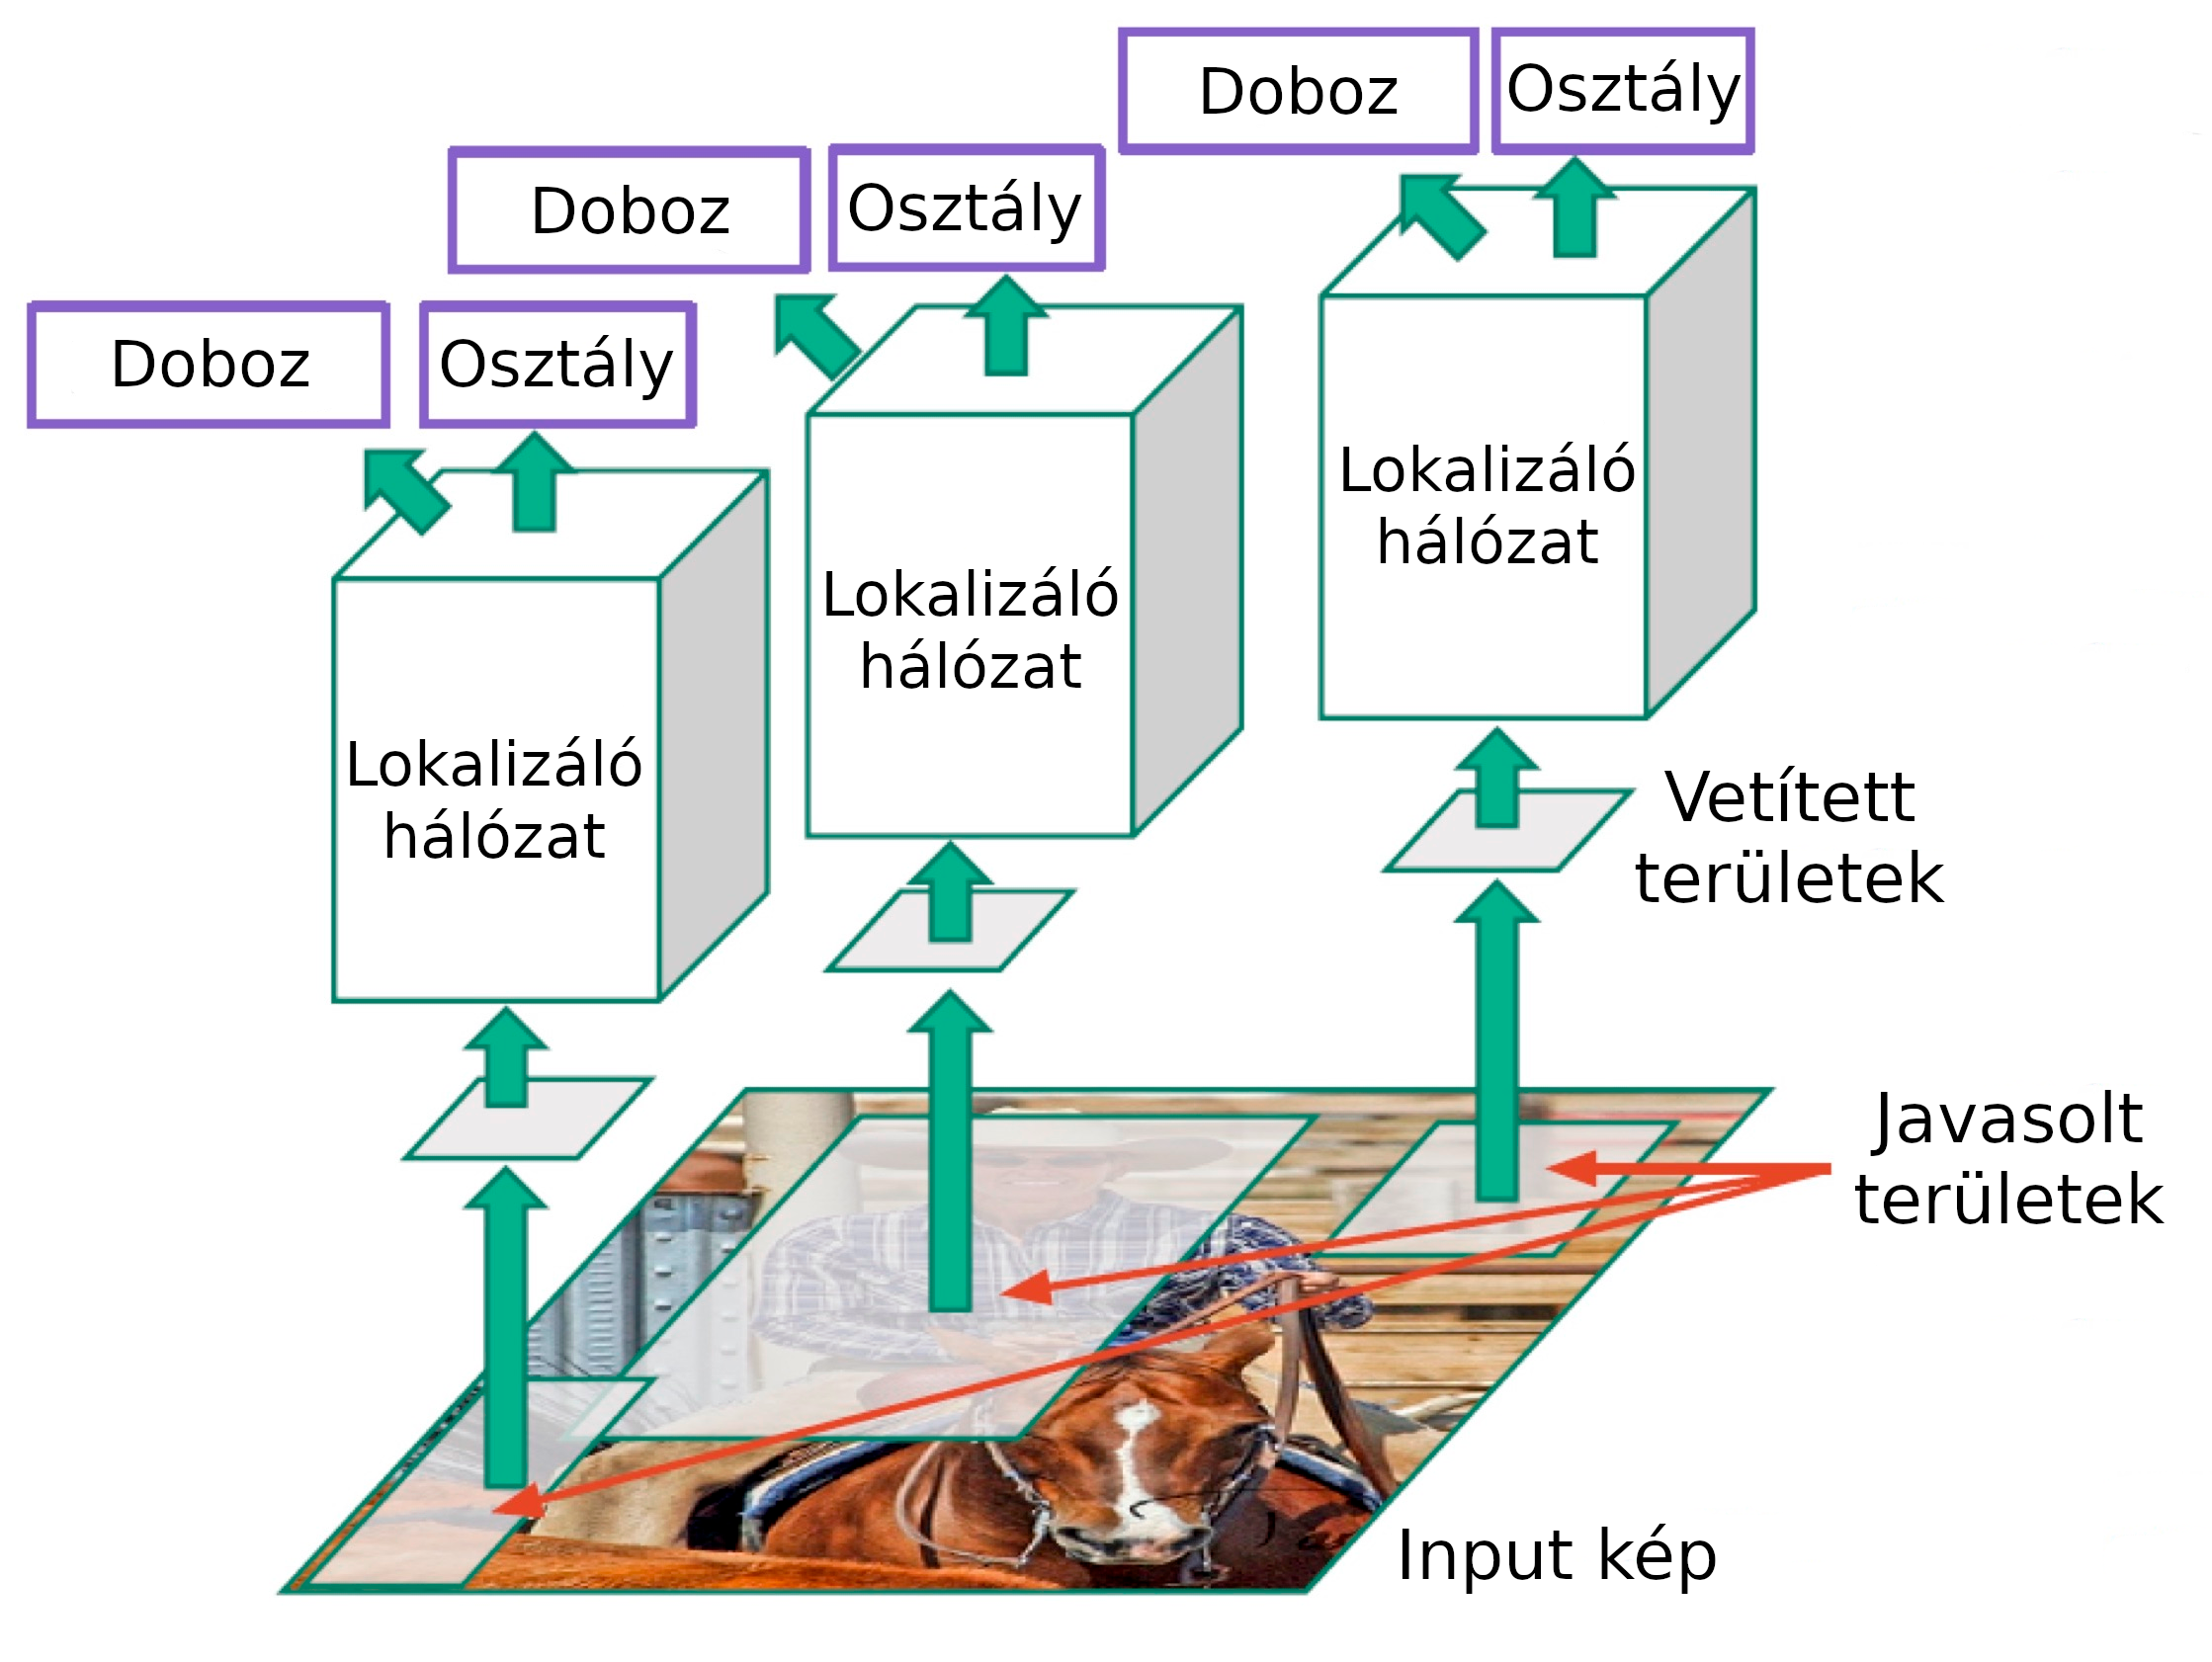
\includegraphics[height=10cm, width=8.5cm, keepaspectratio]{images/od_10.png}}
\end{center}
\end{column}
\end{columns}
\end{frame}

\end{document}








